\documentclass[10pt, a4paper]{article}

\usepackage{ctex}
\usepackage{xeCJK}
\usepackage{caption}
\usepackage{geometry}
\geometry{
    left = 0.6in,
    right = 0.6in,
    top = 0.8in,
    bottom = 1.0in
}
\usepackage{amssymb}
\usepackage{amsbsy}
\usepackage{amsmath}
\usepackage{xcolor}
\usepackage{mathrsfs}
\usepackage{graphicx}
\usepackage{tasks}
\settasks{
    label = \Alph*. ,
    label-width = 16pt
}

\newcommand{\Title}[3]{
    \begin{center}
        \Large \textbf{中国电子学会 #1~年~#2~月 Scratch~#3级考试}
    \end{center}
}
\newcommand{\TimeAndName}[1]{
    \begin{center}
        考试时间:~#1~ 分钟 \qquad\qquad\qquad\qquad 姓名:\underline{\quad\quad\quad\quad}
    \end{center}
}
\pagestyle{empty}
\begin{document}
    \Title{2021}{6}{一}
    
    \TimeAndName{60}
    
    {\noindent\heiti 第一部分、单选题(共 25 题,每题 2 分,共50分.)}

    \begin{enumerate}
        % 1
        \item 小猫位置在舞台中心,点击一次小猫后能前进10步的程序为?(\qquad)
        \begin{tasks}(4)
            \task 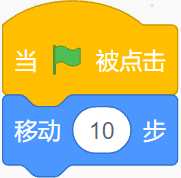
\includegraphics[width=.1\textwidth]{1a.png}
            \task 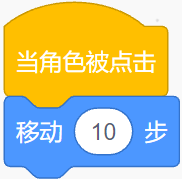
\includegraphics[width=.1\textwidth]{1b.png}
            \task 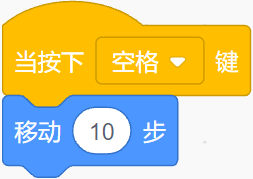
\includegraphics[width=.14\textwidth]{1c.png}
            \task 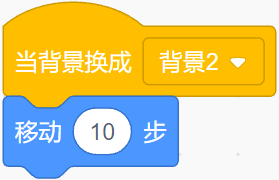
\includegraphics[width=.15\textwidth]{1d.png}
        \end{tasks}

        % 2
        \item 快速切换到下一个背景图片应该使用哪个积木?(\qquad)
        \begin{tasks}(4)
            \task 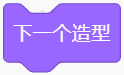
\includegraphics[width=.08\textwidth]{2a.png}
            \task 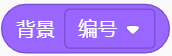
\includegraphics[width=.12\textwidth]{2b.png}
            \task 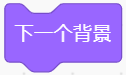
\includegraphics[width=.08\textwidth]{2c.png}
            \task 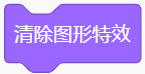
\includegraphics[width=.1\textwidth]{2d.png}
        \end{tasks}

        % 3
        \item 小猫现在面向右,每个格子的边长都是60,请问下面哪段程序不能让小猫走到礼物盒子的位置?(\qquad)
        \begin{tasks}(4)1
            \task 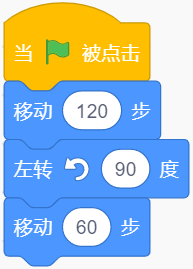
\includegraphics[width=.1\textwidth]{3a.png}
            \task 
\includegraphics[width=.1\textwidth]{3b.png}
            \task 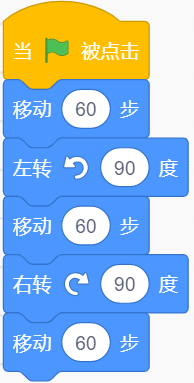
\includegraphics[width=.09\textwidth]{3c.png}
            \task 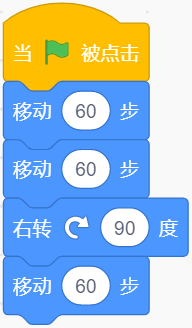
\includegraphics[width=.1\textwidth]{3d.png}
        \end{tasks}

        \begin{figure}[htbp]
            \centering
            \begin{minipage}[t]{.16\textwidth}
                \centering
                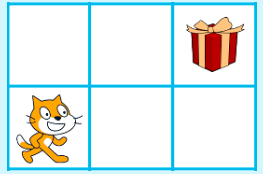
\includegraphics[width=\textwidth]{3.png}
                \caption*{第3题}
            \end{minipage}
            \begin{minipage}[t]{.2\textwidth}
                \centering
                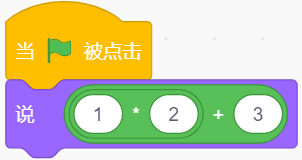
\includegraphics[width=\textwidth]{5.png}
                \caption*{第5题}
            \end{minipage}
            \begin{minipage}[t]{.16\textwidth}
                \centering
                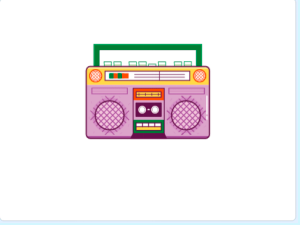
\includegraphics[width=\textwidth]{6.png}
                \caption*{第6题}
            \end{minipage}
        \end{figure}

        % 4
        \item 下面选项中,红色方框正确标出“脚本区”的是?(\qquad)
        \begin{tasks}(4)
            \task 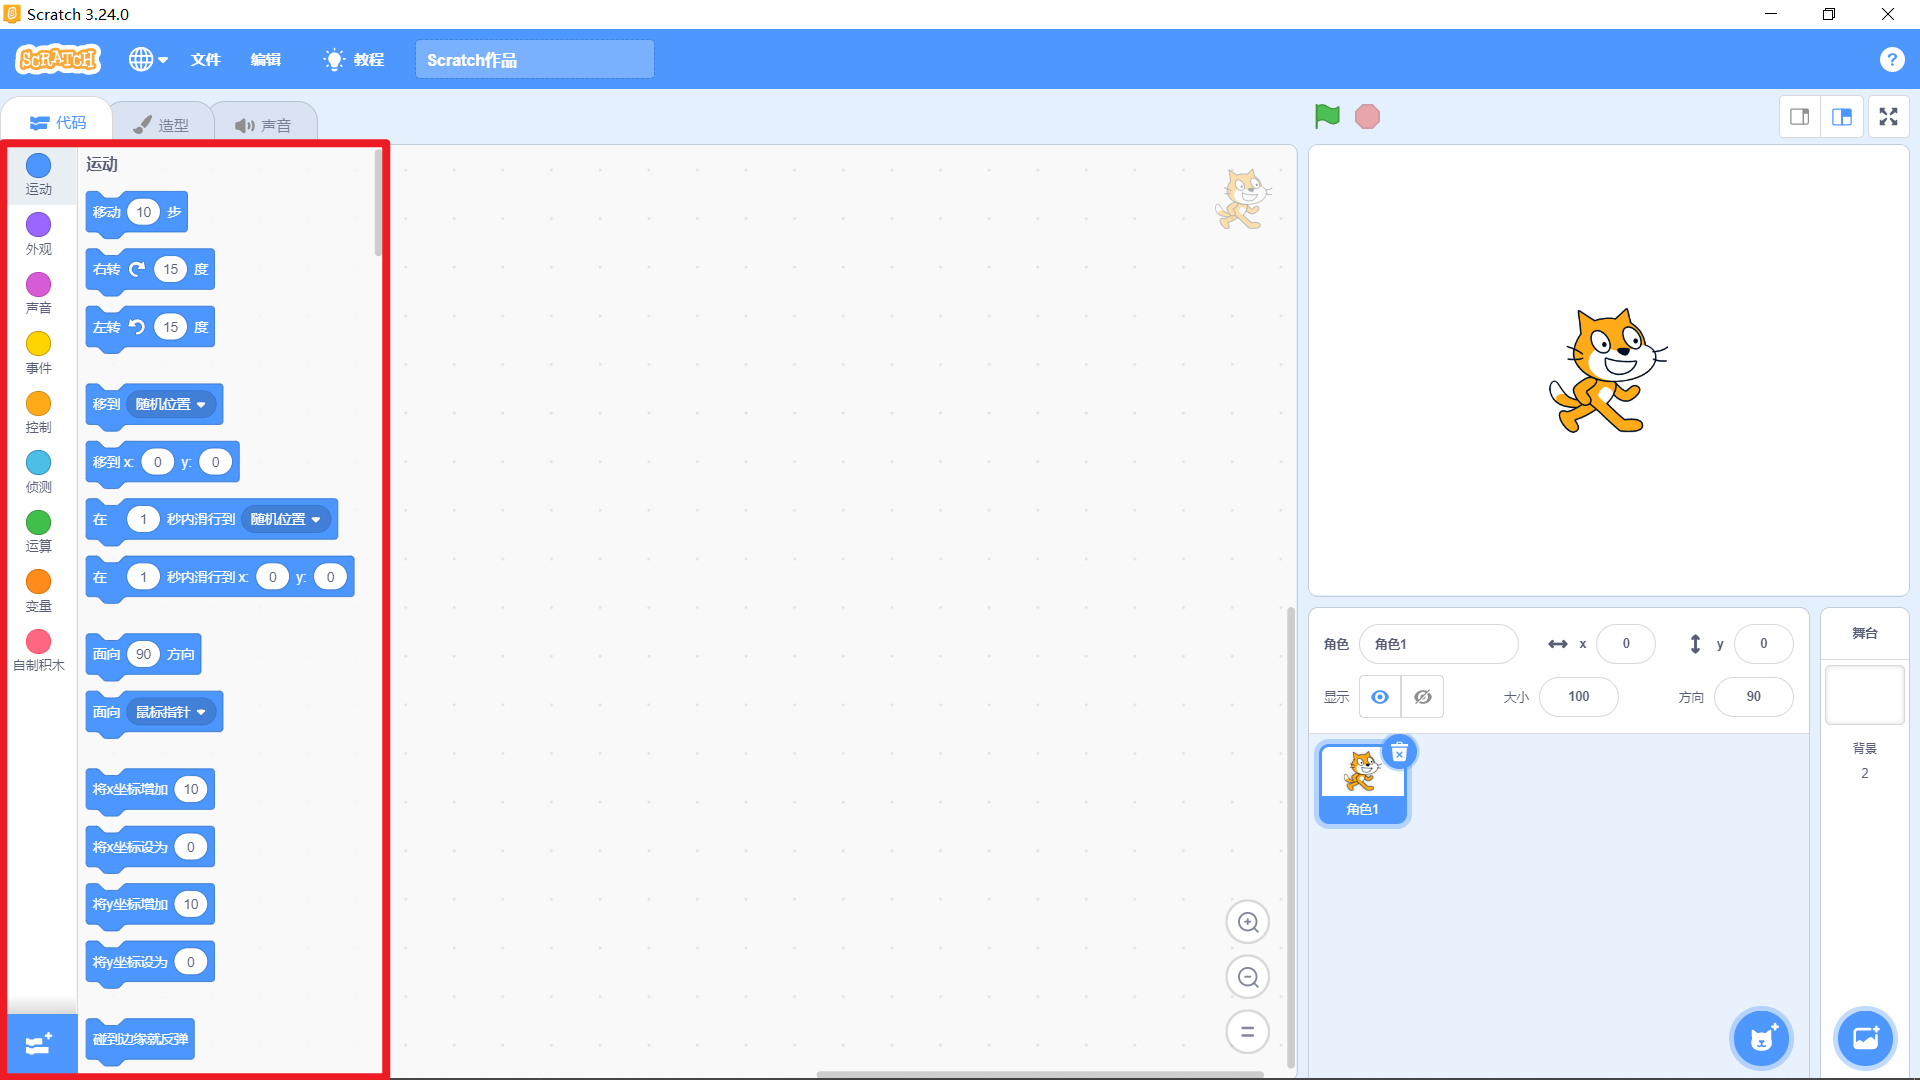
\includegraphics[width=.15\textwidth]{4a.png}
            \task 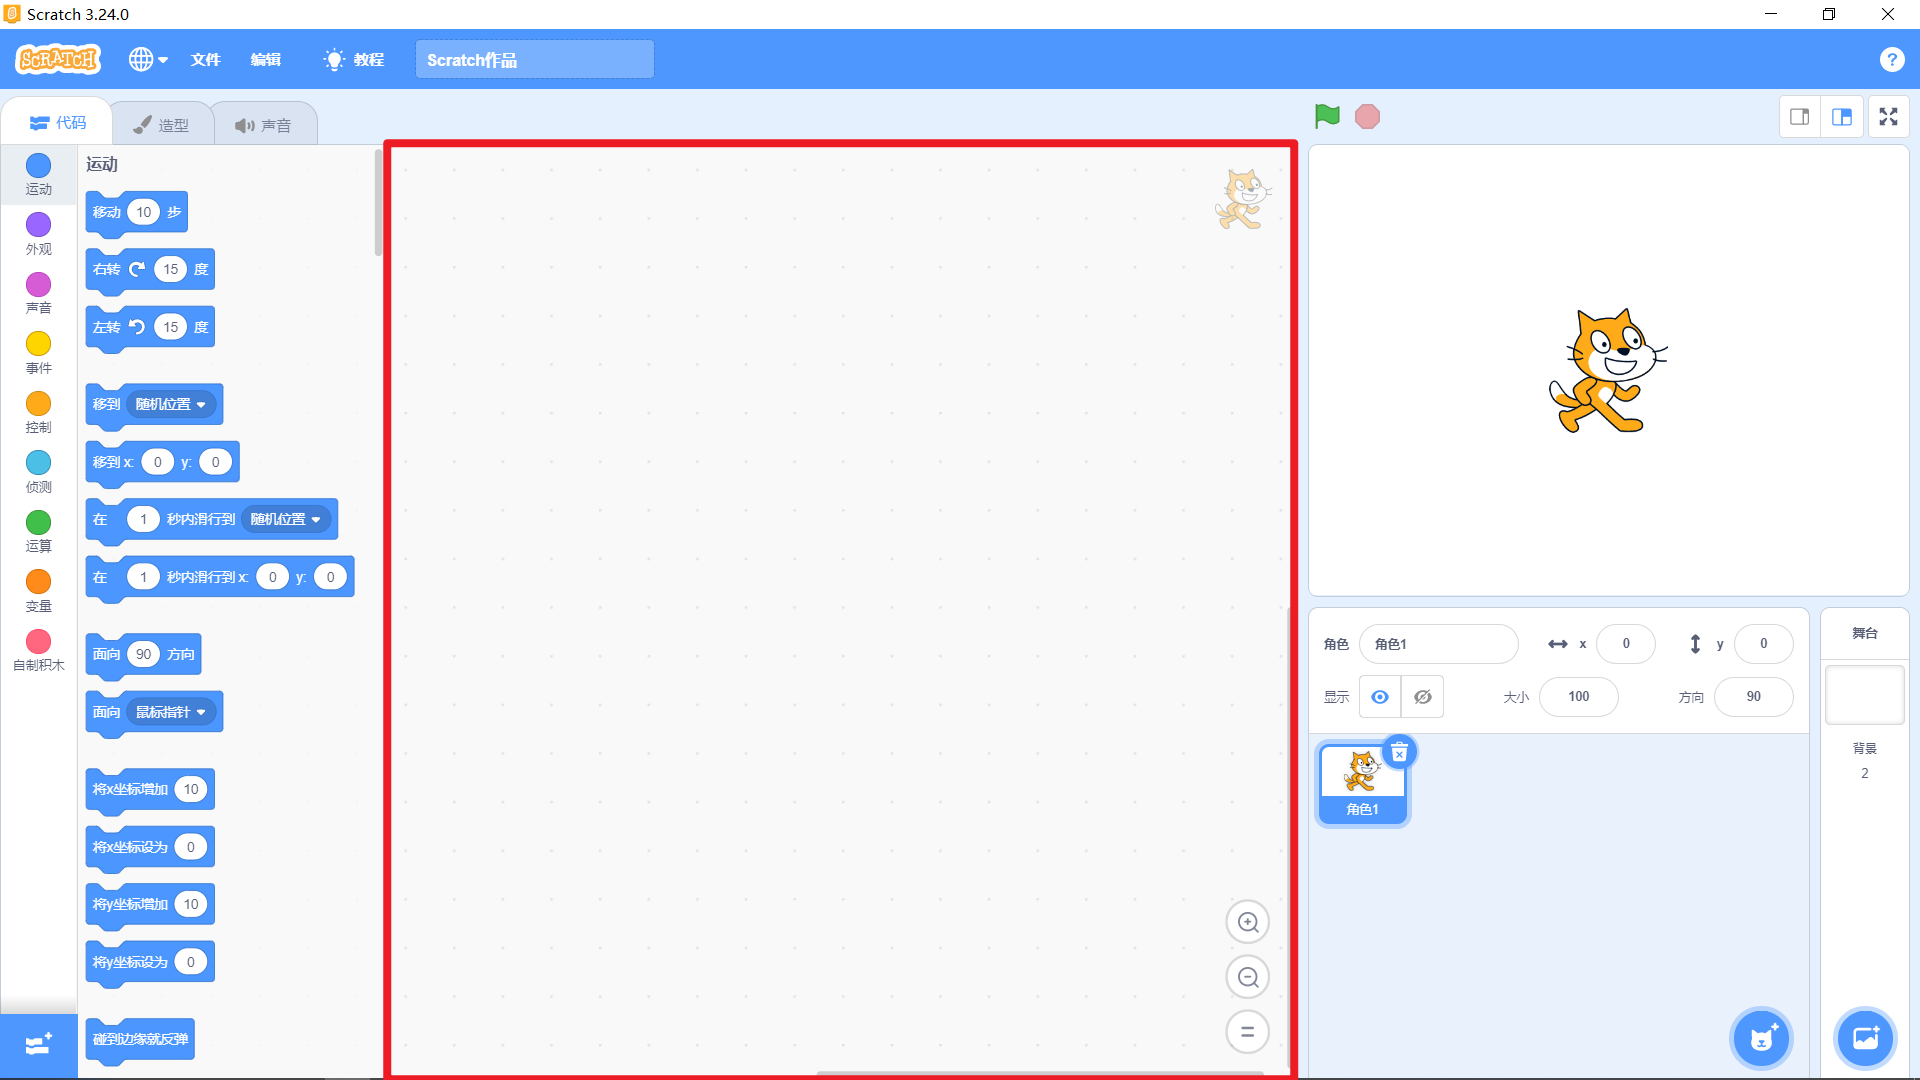
\includegraphics[width=.15\textwidth]{4b.png}
            \task 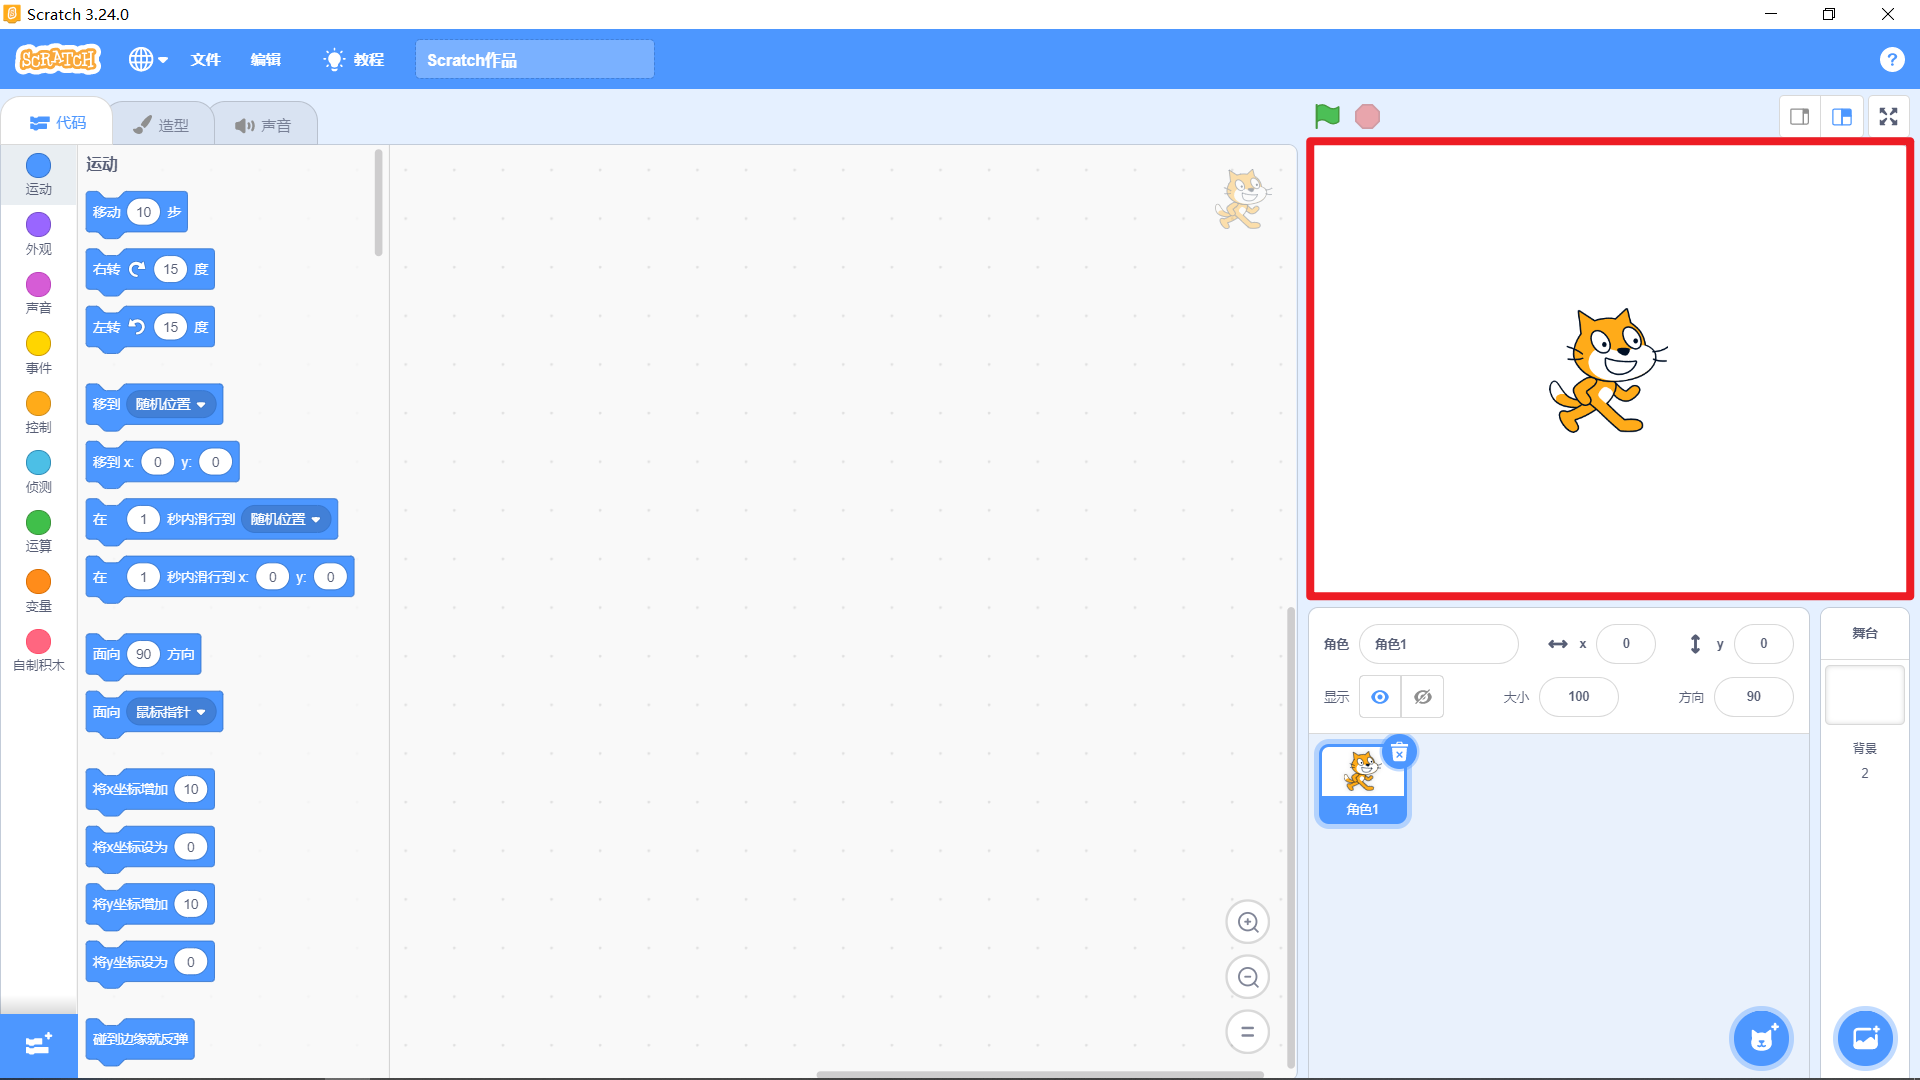
\includegraphics[width=.15\textwidth]{4c.png}
            \task 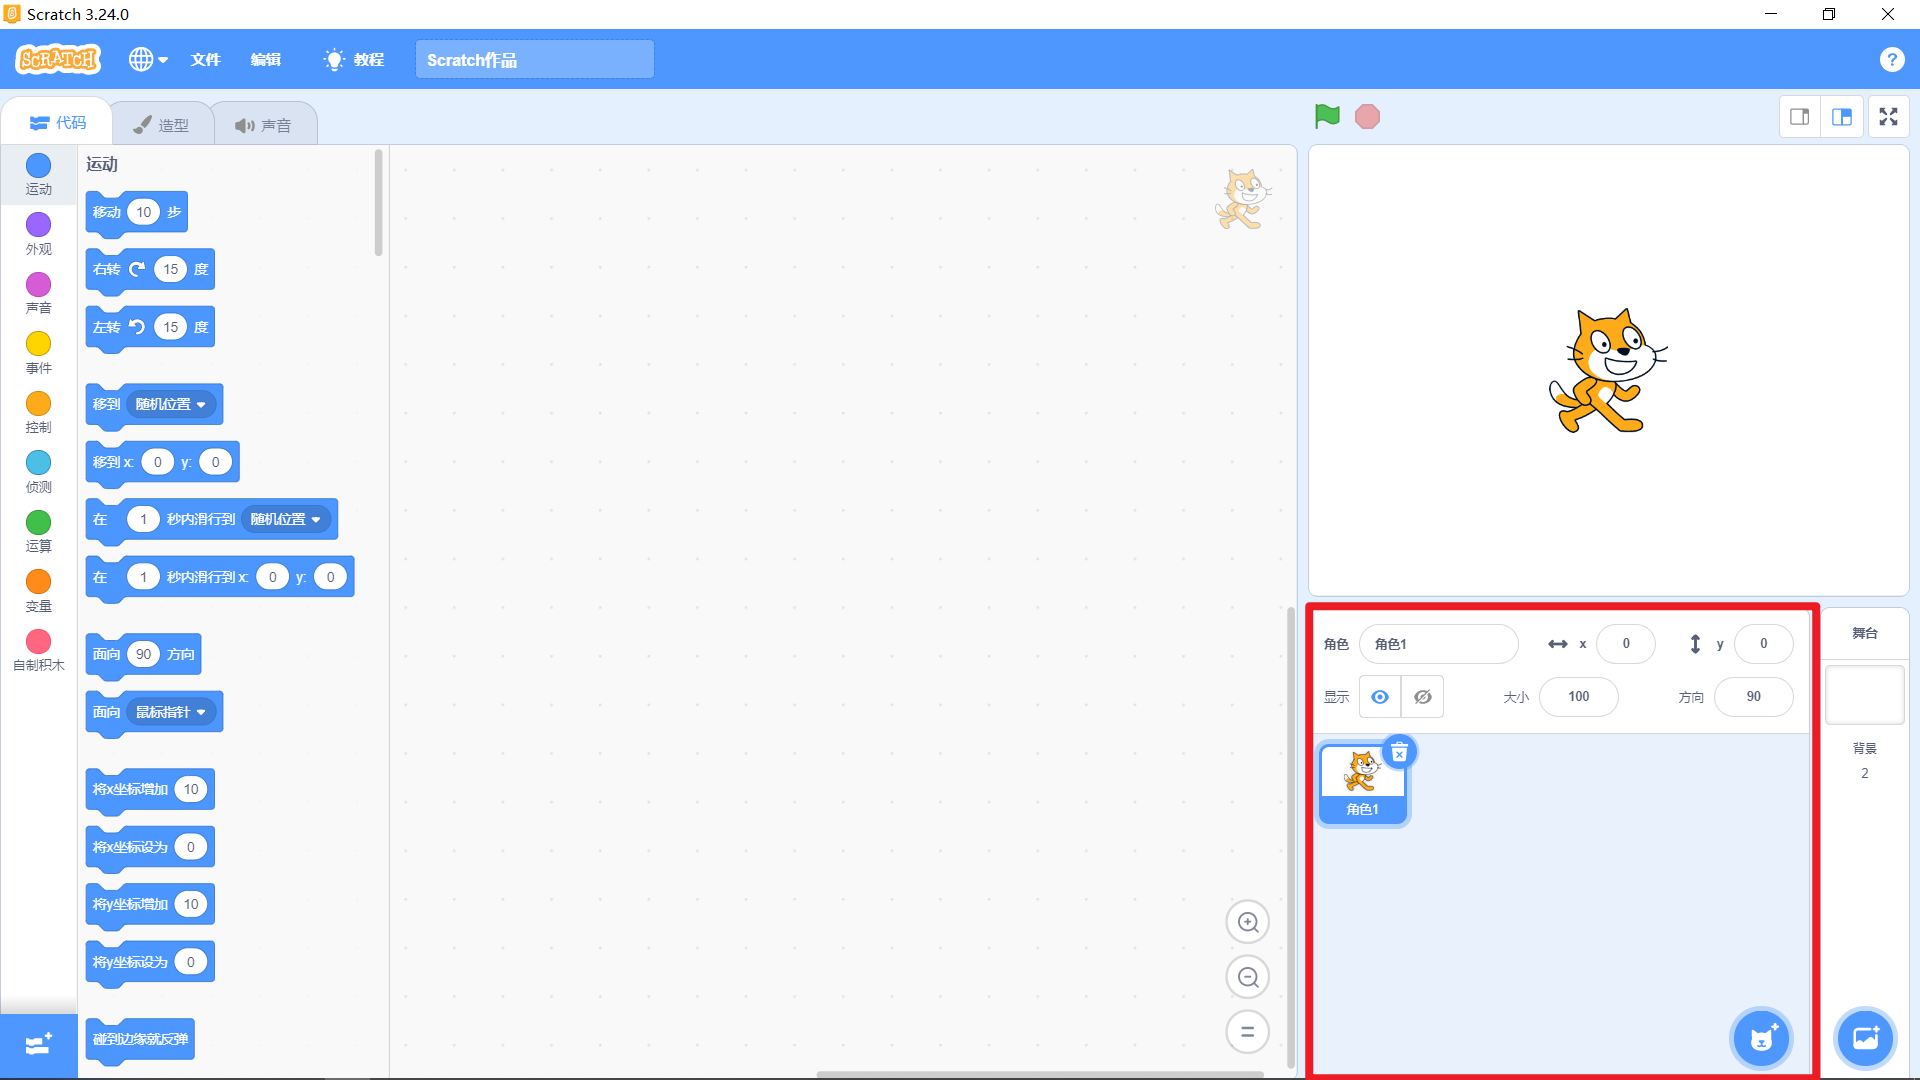
\includegraphics[width=.15\textwidth]{4d.png}
        \end{tasks}

        % 5
        \item 如上图所示,默认小猫角色,运行程序后,显示的数字是?(\qquad)
        \begin{tasks}(4)
            \task 3
            \task 5
            \task 7
            \task 9
        \end{tasks}

        % 6
        \item 音乐Video Game1的时长将近8秒,点击一次角色,下面哪个程序不能完整地播放音乐两次?(\qquad)
        \begin{tasks}(4)
            \task 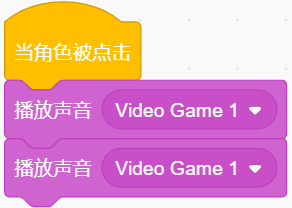
\includegraphics[width=.15\textwidth]{6a.png}
            \task 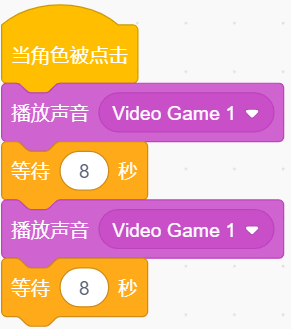
\includegraphics[width=.12\textwidth]{6b.png}
            \task 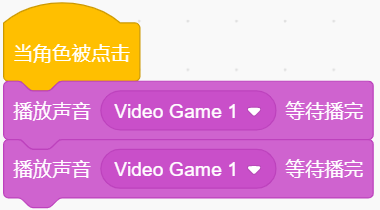
\includegraphics[width=.16\textwidth]{6c.png}
            \task 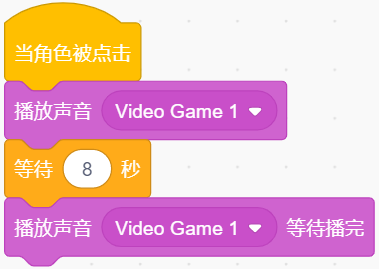
\includegraphics[width=.15\textwidth]{6d.png}
        \end{tasks}
        
        % 7
        \item 有一条长度为500米的马路,马路边每隔1米种着1棵树,路的两端也会种树。由于要修地铁,需要移走距离起点50米到200米、150米到320米和450米到451米区域的树(包括这些区域两端的树)。请问将这些树都移走后,马路上还有多少棵树呢?(\qquad)
        \begin{tasks}(4)
            \task 322
            \task 178
            \task 272
            \task 228
        \end{tasks}
           
        \newpage
        % 8
        \item 默认的小猫,造型和程序如下图所示,点击绿旗,发现看不到小猫迈步的动作,需要增加下面哪个选项的积木,才能看到小猫迈步?(\qquad)
        \begin{tasks}(4)
            \task 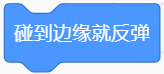
\includegraphics[width=.12\textwidth]{8a.png}
            \task 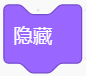
\includegraphics[width=.06\textwidth]{8b.png}
            \task 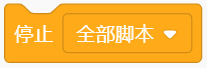
\includegraphics[width=.15\textwidth]{8c.png}
            \task 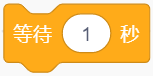
\includegraphics[width=.11\textwidth]{8d.png}
        \end{tasks}

        % 9
        \item 使用下面哪个积木可以设置音调为100?(\qquad)
        \begin{tasks}(4)
            \task 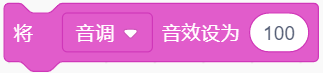
\includegraphics[width=.18\textwidth]{9a.png}
            \task 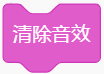
\includegraphics[width=.07\textwidth]{9b.png}
            \task 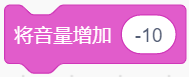
\includegraphics[width=.12\textwidth]{9c.png}
            \task 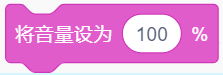
\includegraphics[width=.15\textwidth]{9d.png}
        \end{tasks}

       % 10
       \item 观察下面图片,下面哪个图属于舞台背景中的一部分?(\qquad)
       \begin{tasks}(4)
           \task 
\includegraphics[width=.05\textwidth]{10a.png}
           \task 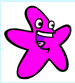
\includegraphics[width=.05\textwidth]{10b.png}
           \task 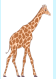
\includegraphics[width=.05\textwidth]{10c.png}
           \task 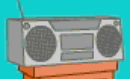
\includegraphics[width=.08\textwidth]{10d.png}
       \end{tasks}

        % 11
        \item 使用下面哪个选项可以将网络搜索到的图片导入作为舞台背景?(\qquad)
        \begin{tasks}(4)
            \task 
\includegraphics[width=.03\textwidth]{11a.png}
            \task 
\includegraphics[width=.03\textwidth]{11b.png}
            \task 
\includegraphics[width=.03\textwidth]{11c.png}
            \task 
\includegraphics[width=.03\textwidth]{11d.png}
        \end{tasks}

        \begin{figure}[htbp]
            \centering
            \begin{minipage}[t]{.23\textwidth}
                \centering
                \begin{minipage}[t]{.5\textwidth}
                    \centering
                    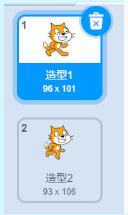
\includegraphics[width=\textwidth]{8-1.png}
                \end{minipage}
                \begin{minipage}[t]{.3\textwidth}
                    \centering
                    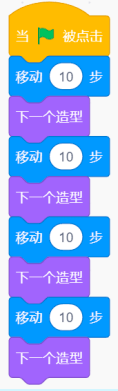
\includegraphics[width=\textwidth]{8-2.png}
                \end{minipage}
                \caption*{第8题}
            \end{minipage}
            \begin{minipage}[t]{.2\textwidth}
                \centering
                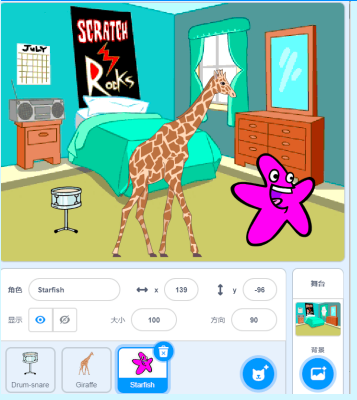
\includegraphics[width=\textwidth]{10.png}
                \caption*{第10题}
            \end{minipage}
            \begin{minipage}[t]{.13\textwidth}
                \centering
                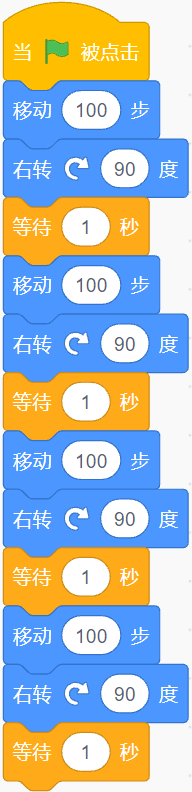
\includegraphics[width=.6\textwidth]{13.png}
                \caption*{第13题}
            \end{minipage}
            \begin{minipage}[t]{.33\textwidth}
                \centering
                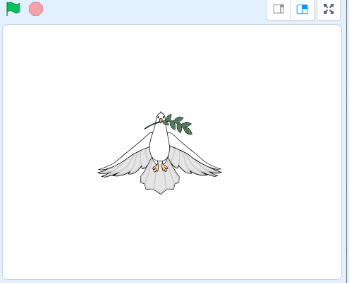
\includegraphics[width=.8\textwidth]{16.png}
                \caption*{第16题}
            \end{minipage}
        \end{figure}
        
        % 12
        \item 下面哪个区域可以更改角色的名字?(\qquad)
        \begin{tasks}(4)
            \task 代码区
            \task 舞台区
            \task 角色列表区
            \task 积木区
        \end{tasks}

       % 13
       \item 默认小猫角色,初始位置在舞台中心,面向右,运行上面程序,小猫走过的图形为?(\qquad)
       \begin{tasks}(4)
           \task 正方形
           \task 三角形
           \task 圆形
           \task 梯形
       \end{tasks}

        % 14
        \item 下面哪个选项可以录入自己的声音?(\qquad)
        \begin{tasks}(4)
            \task 
\includegraphics[width=.03\textwidth]{14a.png}
            \task 
\includegraphics[width=.03\textwidth]{14b.png}
            \task 
\includegraphics[width=.03\textwidth]{14c.png}
            \task 
\includegraphics[width=.03\textwidth]{14d.png}
        \end{tasks}
    
        \item  默认小猫角色播放声音后,执行下面哪个积木,听不到小猫的声音?(\qquad)
        \begin{tasks}(4)
            \task 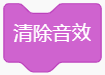
\includegraphics[width=.06\textwidth]{15a.png}
            \task 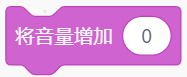
\includegraphics[width=.11\textwidth]{15b.png}
            \task \includegraphics[width=.11\textwidth]{15c.png}
            \task \includegraphics[width=.18\textwidth]{15d.png}
        \end{tasks}
        
        % 16
        \item 如上图,角色白鸽的嘴里衔着一支绿叶,现在想将绿叶去掉,下面哪个选项可以实现?(\qquad)
        \begin{tasks}(4)
            \task \includegraphics[width=.05\textwidth]{16a.png}
            \task \includegraphics[width=.05\textwidth]{16b.png}
            \task \includegraphics[width=.05\textwidth]{16c.png}
            \task \includegraphics[width=.05\textwidth]{16d.png}
        \end{tasks}

        \newpage
        % 17
        \item 使用下面哪个选项的积木可以切换到指定的舞台背景图片?(\qquad)
        \begin{tasks}(4)
            \task \includegraphics[width=.15\textwidth]{17a.png}
            \task \includegraphics[width=.1\textwidth]{17b.png}
            \task \includegraphics[width=.15\textwidth]{17c.png}
            \task \includegraphics[width=.1\textwidth]{17d.png}
        \end{tasks}

        % 18
        \item 点击绿旗,下面哪个选项的程序能让小猫走到蝴蝶处?(\qquad)
        \begin{tasks}(4)
            \task \includegraphics[width=.1\textwidth]{18a.png}
            \task \includegraphics[width=.1\textwidth]{18b.png}
            \task \includegraphics[width=.1\textwidth]{18c.png}
            \task \includegraphics[width=.1\textwidth]{18d.png}
        \end{tasks}

       % 19
       \item 红绿灯角色的造型和程序如下图所示,现在造型为造型1,点击绿旗后,角色会发生什么变化?(\qquad)
       \begin{tasks}(2)
           \task 造型1变为造型2
           \task 造型未发生变化,仍旧是造型1
           \task 造型1和造型2交替切换
           \task 以上都有可能
       \end{tasks}

       \begin{figure}[htbp]
            \centering
            \begin{minipage}[t]{.15\textwidth}
                \centering
                \includegraphics[width=\textwidth]{18.png}
                \caption*{第18题}
            \end{minipage}
            \begin{minipage}[t]{.2\textwidth}
                \centering
                \begin{minipage}[t]{.48\textwidth}
                    \centering
                    \includegraphics[width=\textwidth]{19-1.png}
                \end{minipage}
                \begin{minipage}[t]{.48\textwidth}
                    \centering
                    \includegraphics[width=\textwidth]{19-2.png}
                \end{minipage}
                \caption*{第19题}
            \end{minipage}
            \begin{minipage}[t]{.09\textwidth}
                \centering
                \includegraphics[width=\textwidth]{20.png}
                \caption*{第20题}
            \end{minipage}
            \begin{minipage}[t]{.2\textwidth}
                \centering
                \includegraphics[width=\textwidth]{22.png}
                \caption*{第22题}
            \end{minipage}
            \begin{minipage}[t]{.3\textwidth}
                \centering
                \begin{minipage}[t]{.48\textwidth}
                    \centering
                    \includegraphics[width=\textwidth]{23-1.png}
                \end{minipage}
                \begin{minipage}[t]{.4\textwidth}
                    \centering
                    \includegraphics[width=\textwidth]{23-2.png}
                \end{minipage}
                \caption*{第23题}
            \end{minipage}
        \end{figure}

        % 20
        \item  默认小猫角色的造型如上图所示,实现小猫走动的动画,会用到下面哪个选项中的积木?(\qquad)
        \begin{tasks}(4)
            \task \includegraphics[width=.18\textwidth]{20a.png}
            \task \includegraphics[width=.1\textwidth]{20b.png}
            \task \includegraphics[width=.15\textwidth]{20c.png}
            \task \includegraphics[width=.08\textwidth]{20d.png}
        \end{tasks}

        % 21
        \item 添加新的舞台背景图片,应该点击下面哪个选项?(\qquad)
        \begin{tasks}(4)
            \task \includegraphics[width=.04\textwidth]{21a.png}
            \task \includegraphics[width=.04\textwidth]{21b.png}
            \task \includegraphics[width=.04\textwidth]{21c.png}
            \task \includegraphics[width=.04\textwidth]{21d.png}
        \end{tasks}

        % 22
        \item 运行上面程序,小猫会说出哪个数字?(\qquad)
        \begin{tasks}(4)
            \task 18
            \task 20
            \task 24
            \task 14
        \end{tasks}

        % 23
        \item 舞台和昆虫的程序如上图所示,鼠标点击昆虫三次后,触角朝向哪个方向?(\qquad)
        \begin{tasks}(4)
            \task 舞台左侧
            \task 舞台右侧
            \task 舞台上方
            \task 舞台下方
        \end{tasks}

        % 24
        \item 小风用Scratch为《静夜思》设计了一段动画,在运行作品的过程中他发现动画还有问题,请问他应该点击哪个按钮停止作品运行,修改程序?(\qquad)
        \begin{tasks}(4)
            \task \includegraphics[width=.04\textwidth]{24a.png}
            \task \includegraphics[width=.04\textwidth]{24b.png}
            \task \includegraphics[width=.05\textwidth]{24c.png}
            \task \includegraphics[width=.05\textwidth]{24d.png}
        \end{tasks}
        
        % 25
        \item 下面哪个选项可以实现增加一个新角仓?(\qquad)
        \begin{tasks}(4)
            \task 从角色库导入
            \task 自己绘制一个角色
            \task 通过本地电脑导入
            \task 以上三个都可以
        \end{tasks}
    \end{enumerate}

    \newpage
    {\noindent\heiti 第二部分、判断题(共 10 题,每题 2 分,共20分.)}
    \begin{enumerate}
        \setcounter{enumi}{25}
        % 26
        \item 角色的造型和背景可以在矢量图与位图间进行转换.(\qquad)

        %27
        \item 角色导入后用图形编辑器中的工具进行编辑,可以对原角色造型进行修改.(\qquad)
        
        %28
        \item 停止播放声音,只能使用\includegraphics[width=.1\textwidth]{28.png}所示积木.(\qquad)
  
        %29
        \item 舞台中的角色默认面向0度方向.(\qquad)
        
        %30
        \item Scratch的默认小猫角色,一开始默认面向90度方向,也就是面向右.(\qquad)

        %31
        \item 可以导入网上下载的音乐作为程序中的声音.(\qquad)
        
        %32
        \item 系统自带的角色、背景素材只能导入无法修改.(\qquad)
        
        %33
        \item 将Scratch3程序文件保存到电脑上,文件后缀名为.sb3.(\qquad)
        
        %34
        \item 可以复制角色的矢量图造型来生成新造型,也可以使用缩放,旋转,绘制等工具修改该造型.(\qquad)
        
        %35
        \item 可以通过程序来控制角色行进方向和距离.(\qquad)
    \end{enumerate}

    {\noindent\heiti 第三部分、编程题(共 2 题,共30分.)}
    \begin{enumerate}
        \setcounter{enumi}{35}
        
        % 36
        \item 奔跑的马:
        
        1. 准备工作
        \begin{tasks}[label = (\arabic*)]
            \task 添加背景Forest和Wetland;
            \task 添加角色Unicorn Running;
            \task 为Unicorn Running添加声音Gallop.
        \end{tasks}
        2. 功能实现
        \begin{tasks}[label = (\arabic*)]
            \task 点击绿旗,角色Unicom Running的初始位置在舞台左边,初始背景为Forest;
            \task 角色Unicom Running切换着造型向右跑;
            \task 角色Unicom Running跑到舞台右侧边缘,背景切换为Wetland,折返跑向舞台左侧;
            \task 角色Unicom Running跑到舞台左侧边缘后,播放声音Gallop.
        \end{tasks}

        \begin{center}
            \includegraphics[width=.4\textwidth]{36.png}
        \end{center}

        %37
        \item 打篮球:
        
        1. 准备工作
        \begin{tasks}[label = (\arabic*)]
            \task 添加背景 Basketball2;
            \task 添加角色Hannah;
            \task 为角色添加Hannah声音cheer.
        \end{tasks}
        2. 功能实现
        \begin{tasks}[label = (\arabic*)]
            \task 当绿旗被点击,角色Hannah初始位置在舞台的右侧,造型为hannah-a;
            \task 按下空格键,角色Hannah向左跑到篮筐下;
            \task 点击角色Hannah,切换到hannah-c造型向上跳起投篮,播放声音cheer,声音播完后,落回地面,造型切换到hannah-D。
        \end{tasks}

        \begin{figure}[htbp]
            \centering
            \begin{minipage}{.3\textwidth}
                \centering
                \includegraphics[width=\textwidth]{37-1.png}
            \end{minipage}
            \begin{minipage}{.3\textwidth}
                \centering
                \includegraphics[width=\textwidth]{37-2.png}
            \end{minipage}
            \begin{minipage}{.3\textwidth}
                \centering
                \includegraphics[width=\textwidth]{37-3.png}
            \end{minipage}
        \end{figure}
    \end{enumerate}
\end{document}